\section{The population section\label{sec:population-section}}

\subsection{Overview}

The spatial structure of \SPM\ is represented by an $n \times m$ grid, with rows $i=1 \dots n$ and columns $j=1 \ldots m$. Each cell of this matrix records the population structure at that point in space and is represented by an $k \times l$ rectangular matrix (with categories $k=1 \ldots k$ and ages $l=age_{min} \ldots age_{max}$. Hence we can describe any spatial and population element of the model as element$(i,j,k,l)$. 

\subsection{Spatial structure}

The spatial structure of \SPM\ is represented by an $n \times m$ grid, with rows $i=1 \dots n$ and columns $j=1 \ldots m$. Each cell of this matrix records the population structure at that point in space and is represented by an $k \times l$ rectangular matrix (with categories $k=1 \ldots k$ and ages $l=age_{min} \ldots age_{max}$. Hence we can describe any spatial and population element of the model as element$(i,j,k,l)$. 

\SPM\ implements two spatial structures, \emph{square} \textemdash the default (see Figure \ref{fig:SquareSpatialStructure}) and \emph{hexagon} (see Figure \ref{fig:HexagonSpatialStructure}). These effect the location of neighbours (for adjacent movements), and the distance between cells. For a square grid, the distance between any cell a and cell b is defined as,

\[
d\left( {a,b} \right) = \lambda \sqrt {\left( {x_a  - x_b } \right)^2  + \left( {y_a  - y_b } \right)^2 } 
\]

where $x$ and $y$ represent the x- and y-coordinates of $a$ and $b$ respectively, and $\lambda$ is an arbitrary scalar representing the length of one side of the square.

For a hexagonal grid, the distance between cell a and cell b is defined as,

\[
d\left( {a,b} \right) = \lambda \sqrt {\left( {x_a  - x_b } \right)^2  + \left( {y_a  - y_b } \right)^2 } 
\]

where $x$ and $y$ represent the x- and y-coordinates of $a$ and $b$ respectively, and $\lambda$ is an arbitrary scalar representing the length of one side of the hexagon. 

Note that under these definition, the distance between any cell and itself is 0.


\begin{figure}[htp]
\resizebox{\textwidth}{!}{\includegraphics[width=\textwidth]{Figures/SquareStructure}}
 \caption{The \emph{square} spatial structure}
 \label{fig:SquareSpatialStructure}
\end{figure}

\begin{figure}[htp]
\resizebox{\textwidth}{!}{\includegraphics[width=\textwidth]{Figures/HexagonStructure}}
 \caption{The \emph{hexagon} spatial structure}
 \label{fig:HexagonSpatialStructure}
\end{figure}

\subsection{Population structure}

The population structure in \SPM\ is represented by a matrix containing an arbitrary number of user defined categories (rows), and an arbitrary age range (columns). Hence, each spatial cell has a population state described as $n_{categories} \times n_{ages}$ rectangular matrix with categories $k=1 \ldots n_{categories}$ and ages $l=age_{min} \ldots age_{max}$. 

\subsubsection*{Movement processes}

Movement processes are those processes that move individuals between cells but retain the their population state, and are defined such that,

$element(i,j,k,l)\leftarrow element(i,j,k,l) + p \cdot element(i',j',k,l)$,

i.e., each element in cell$(i,j)$ is updated as the sum of itself and some proportion $p$ of a neighbouring element in cell$(i',j')$. To conserve abundance we also update element$(i',j',k,l)$ as,

$element(i',j',k,l)\leftarrow element(i',j',k,l) - p\cdot element(i',j',k,l)$

\SPM\ assumes that each movement process occurs simultaneously over all cells (synchronous updating), i.e., all cell updates from each individual movement process are first evaluated for all cells, and then applied to all cells affected. The movement process (labelled directed movement in \SPM) allows movement from any $cell(a) \rightarrow cell(b)$, for $\forall a,b \in L_B$ and is implemented as a function of the product of up to $n$ independent \emph{preference functions}. We define the probability of moving from any cell $a$ to any cell $b$, for all $a,b \in L_B$, as a function of the relative preference for that cell. See Section \ref{sec:population-section} for detail.
\subsection{Layers}

Within \SPM, layers are used in three contexts:

\begin{enumerate}

\item The base layer: The base layer $L_B$ is a special layer (there must be exactly one base layer defined within the model) that defines the locations where the population can and cannot potentially be present (e.g., locations associated with the sea and not land in a marine model). Here, we define that a cell may potentially have part of the population present if $L_B(i,j) > 0$. Further, positive values of the base layer $L_B$ represent the relative or absolute \emph{area} represented by that spatial cell. 

\item Covariate layers: A model may have many covariate layers, and these are used as covariates of some population or movement process (e.g., sea floor depth may be a covariate of some movement process). The values in layers used as covariates must be continuous (i.e., numeric) variables. Covariate layers must be positive and $\geq 0$.

\item Classification layer. A model may have many classification layers, and these are used as a classification or grouping variable for aggregating data over individual spatial cells $(i,j)$, e.g., statistical areas or management areas. Such layers are typically used to aggregate the population within cells into groups so-as to allow comparison with observations. The values in layers used as classification layers must be categorical variables.

\end{enumerate}

Typically, layers are supplied by the user and are assumed known and constant.However, there are two exceptions to this rule \textemdash layers of type abundance and distance are calculated automatically by \SPM\ as required. For the distance layer, the distance between cell $a$ and cell $b$ is defined as,

$d(a,b)=\sqrt{(x_a-x_b)^2 +(y_a-y_b)^2}$

where $x$ and $y$ represent the x- and y-coordinates of $a$ and $b$ respectively.

For the abundance layer, the abundance of a cell is simply a count of the number of individuals in the cell a within categories $K$, with selectivity $S$,

$N(a)=\sum_{k\in K} \sum_i element(i,j,k,l)$

Note that \SPM\ does not `edit' or otherwise change layers, including adding or otherwise combining layers that are supplied in the input parameter files \textemdash except for a single case for covariate layers. In that instance, the covariate layer supplied can be can optionally (unless of type category or abundance) be standardized prior to use, i.e.,

$L'(a)=L(a)/max(L)$

i.e., $L'(a) < 1$.

\subsection{Initialization}

The annual cycle in \SPM\ consists of an arbitrary number of time steps, and within each time step an arbitrary number of population processes are followed by an arbitrary number of movement processes. 

initialization\_phases Phase1
run\_years 14
start\_year 1994
projection\_years 100

\subsection{Model initialization}

\SPM\ initializes the initial equilibrium state as an iterative process, because a general solution that initializes complex structured movement models can be difficult to implement using analytic techniques. However, initializing via iteration for a long-lived species with complex movements can also be slow to run. In \SPM, we allow for user-defined multi-phased initialization using iteration to allow the user to optimize models for speed. Each phase of the initialization can involve any number of population and/or movement processes. 

Following initialization, the model then runs over a number of user-defined years. For this part of the model, the annual cycle can be broken into separate time steps, and observations can be associated with the state of the model at the end of any time step, i.e., likelihoods for particular observations are evaluated, if required, at the end of each time step. This differs from the more usual implementation (see, for example, Bull et al. 2008) where observations can be associated with the population state during some part of a time step. 

\subsection{Annual cycle}

\subsection{Time steps}

\subsection{Movement processes}

\subsubsection{Directed movement}

\begin{figure}[htp]
\resizebox{\textwidth}{!}{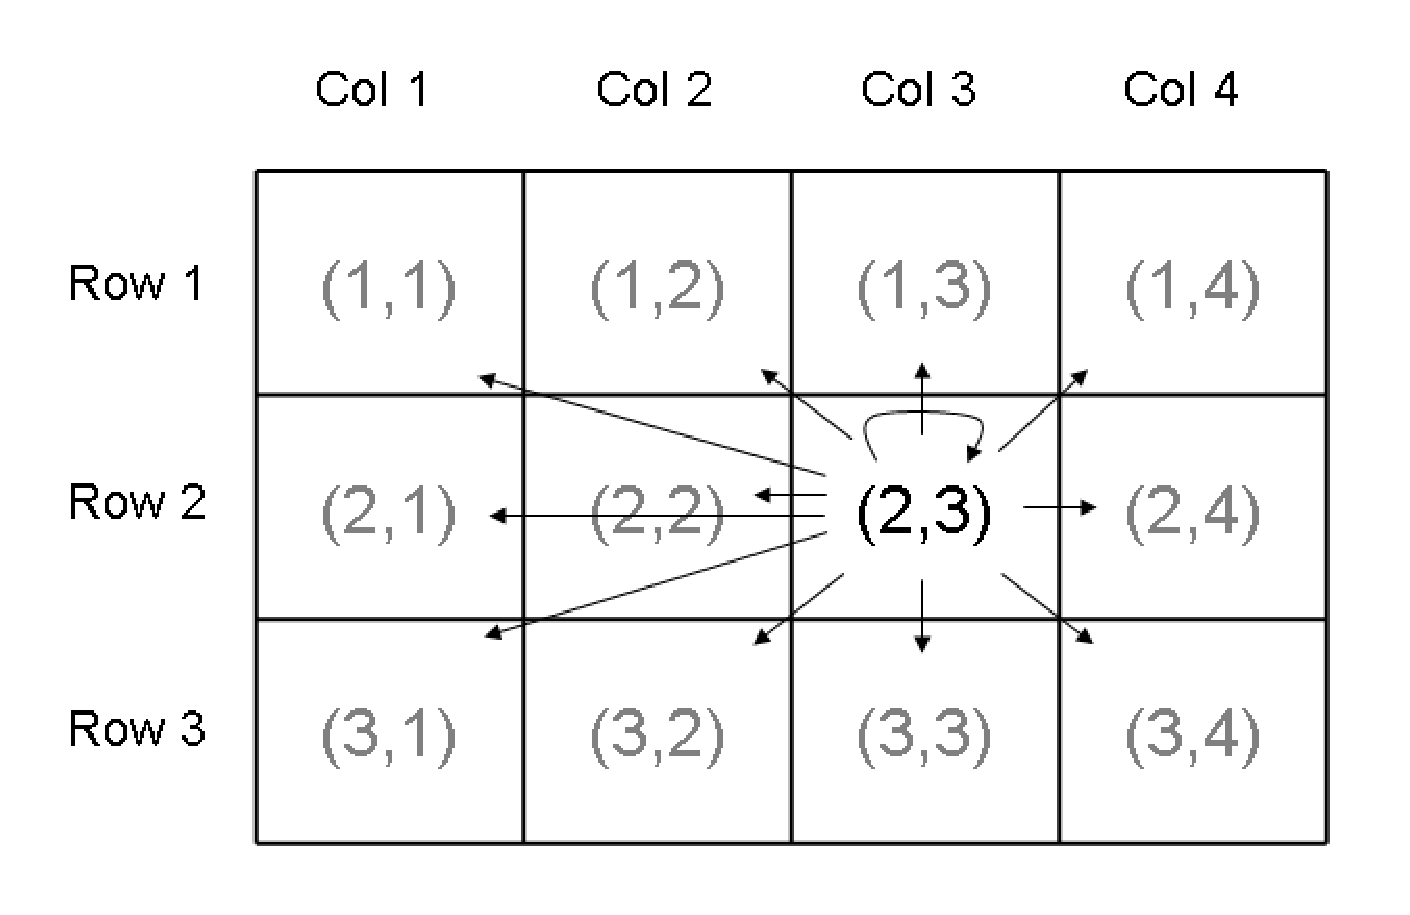
\includegraphics[width=\textwidth]{Figures/Movement}}
 \caption{Movement}
 \label{fig:Movement}
\end{figure}


\paragraph{The preference function}

 Movement in \SPM\ can be defined as a probability distribution based on an underlying preference function. Here, We define the preference for a cell $x$ as the preference function $f_x(\theta_x,P(x))$, where $\theta_x$ are the parameters for $f_x$. So, given a set of $n$ attributes for cell $x$, we can define a preference function for each, and hence we define the aggregated or total preference function for any cell $x$ as the weighted product of individual preference functions,

$P_x=f_1(\theta_1,P_1(x))^{\alpha_1} + f_2(\theta_2,P_2(x))^{\alpha_2} + f_3(\theta_3,P_3(x))^{\alpha_3} + \cdots + f_n(\theta_n,P_n(x))^{\alpha_n}$

where $\alpha_i$ is an arbitrary weighting factor for attribute $i$.

Then we define the probability of moving from cell $a$ to any cell $b$ (where $b$ is defined as the set of all possible cells, including $a$),

$p(a\rightarrow b) = {P_a} / {\sum_{i \in \forall b}P_i}$

Note that there are three forms of preference function,
\begin{enumerate}
\item Those that are a function of some underlying attribute of a cell, as defined by some arbitrary layer $L$
\item Those that are a function of the abundance (perhaps with a selectivity and for a subset of all categories) of each cell
\item Those that are a function of the distance between the sink and the source cells. 
\end{enumerate} 

Preference functions of the first type are determined only by the parameters of the preference function and some underlying, fixed, attribute. Preference functions of the other are dynamic, i.e. they depend on the relative locations of the cells or on the density of a cell at a particular point in time.

\paragraph{Preference functions}

Preference functions in \SPM\ include \subcommand{constant}, \subcommand{normal}, \subcommand{double-normal}, \subcommand{logistic}, \subcommand{inverse-logistic}, \subcommand{exponential-decay}, and \subcommand{threshold}. These are defined as,

\begin{enumerate}
\item The \subcommand{constant}\ preference function has dependent variable $x$ and has no parameters, and is defined as,

$f(x)=x$, where $0 \leq x \leq 1$

\item The \subcommand{normal}\ preference function has dependent variable $x$ and parameters $\theta = (\mu,\sigma)$, and is defined as, 

$f(x | \mu, \sigma) = 2^{-[(x- \mu)/\sigma ]^2} $
 
\item The \subcommand{double-normal}\ preference function has dependent variable $x$ and parameters $\theta=(\mu,\sigma_L,\sigma_R)$, and is defined as,

$f(x | \mu, \sigma_L, \sigma_R) = \left\{ 
\begin{array}{l l}
  2^{-[(x- \mu)/\sigma_L ]^2} & \quad \mbox{if $x \leq \mu$}\\
  2^{-[(x- \mu)/\sigma_R ]^2} & \quad \mbox{if $x \ge \mu$}\\
\end{array} \right.$ 

\item The \subcommand{logistic}\ preference function has dependent variable $x$ and parameters $\theta = (a_{50},a_{to95})$, and is defined as,

$f(x | a_{50}, a_{to95}) = 1 / [1+19^{(a_{50}-x)/a_{to95}}]$

\item The \subcommand{inverse-logistic}\ preference function has dependent variable $x$ and parameters $\theta = (a_{50},a_{to95})$, and is defined as,

$f(x | a_{50}, a_{to95}) =1- 1 / [1+19^{(a_{50}-x)/a_{to95}}]$

\item The \subcommand{exponential-decay}\ preference function has dependent variable $x$ and parameters $\theta = (\lambda)$, and is defined as,

$f(x | \lambda) =\exp(-\lambda x)$, where $x \geq 0$ and $0$ otherwise

\item The \subcommand{threshold}\ preference function has dependent variable $x$ and parameters $\theta = (N,\lambda)$, and is defined as,

$f(x | N, \lambda) = \left\{ 
\begin{array}{l l}
  1 & \quad \mbox{if $x \leq N$}\\
  1/\left({\frac{x}{N}}^\lambda\right) & \quad \mbox{if $x \ge N$}\\
\end{array} \right. $, where $x \geq 0$ and $0$ otherwise

\end{enumerate}

\subsection{Model years}

\subsection{Population processes}

\subsubsection{Recruitment}

\subsubsection{Ageing}

\subsubsection{Mortality}

\subsubsection{Category transitions}

\subsection{Movement processes}

\subsubsection{Directed movement}

\paragraph{Directed-process}

\subsection{Layers}

\subsubsection{Numeric layers}

\subsubsection{Category layers}

\subsubsection{Abundance layers}

\subsubsection{Biomass layers}

\subsubsection{Density layers}

\subsubsection{Distance layers}

\subsection{Selectivity}

\subsubsection{Logistic}

\subsubsection{Logistic producing}

\subsubsection{Knife edge}

\subsubsection{Double normal}

\subsubsection{Constant}


etc.,
